\cleardoublepage
\chapter{Introduction to standing waves and HIFI}
Standing waves are a result from interferences, and interferences are a consequence of coherence.

\section{Coherence and interference}
The mixer receives power from many sources:
\begin{itemize}
    \item the LO signal, high power phase-locked monocromatic, reference of the phases, coherent by design;
    \item the sky signal in both sidebands, a priori incoherent;
    \item noise from the LO, a priori incoherent;
    \item black body radiation from the calibration loads, a priori incoherent;
    \item other sources of noise, thermal or not, a priori incoherent.
\end{itemize}
A priori the useful LO signal is coherent and all the other sources behave like noise.
However, the high frequency resolution of the instrument makes these noise sources coherent.

The coherence time~$\tau$ of a signal is inversely proportional to its bandwidth~$\Delta f$:
the narrower the bandwidth, the longer the signal remains in phase, as illustrated by \cref{fig:coherence}.
\begin{figure}[hbtp]
    \centering
    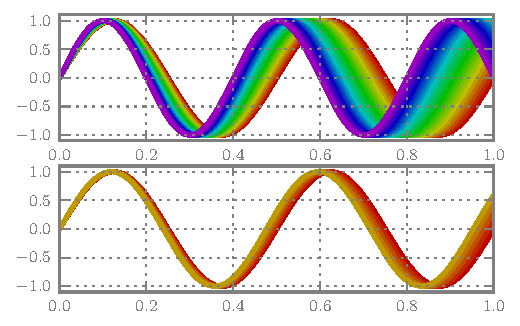
\includegraphics{coherence}
    \caption{
        Signals with a narrow bandwidth remain in phase longer.
        Colors represent frequencies.
        The $x$ axis can represent either time or space and the $y$ axis represents the amplitude of the electric field for the corresponding frequency.
        After propagating to $x=0.85$, the red and purple frequencies of the top-plot signal have opposite phase; a detector that cannot discriminate between them adds up their contribution to 0.
        In the bottom plot, the signal is still very much in phase at $x=0.85$
        because it has a narrower bandwidth.
    }
    \label{fig:coherence}
\end{figure}

Each WBS channel has a bandwidth $\Delta f = \SI{1.1}{\mega\hertz}$,
which yields $\tau = 1 / \Delta f = \SI{909}{\nano\second}$.
By multiplying by the speed of light, we find that the WBS has a coherence length of~\SI{273}{\meter}.
This means that, as long as a signals travels significantly less than~\SI{273}{\meter}, it is coherent as far as the WBS is concerned.
The pathlengths inside HIFI are much shorter than~\SI{273}{\meter}.
For example, the distance between the LOs and the mixers are about~\SI{1}{\meter}.
In that context, all the sources of noise in HIFI are coherent.

Coherence makes you care about the phase, and also about the polarization.

Explain interference.

Show that incoherent systems do not have to care.
Incoherent system: no phase information, just power.
Incoherent system can still have polarization, but they can be unpolarized.
Coherent system are always polarized.






\section{Cavities}
Two reflective surfaces facing each other form a cavity.
At least one of the two surfaces must be partly transparent so that the light can enter and exit the cavity.
The light that enters the cavity can come out after any number $N$ of round trips.
If the distance between the surfaces is $d$, the length of a round trip is $2d$.
After $N$ round trips, a wave of wavelength $\lambda$ is dephased by $2\pi N2d/\lambda$ radians.

The wave inside the cavity is a superposition of the infinite number of waves traveling in both directions (for $N=1$ to $\infty$).
That wave is a ``standing wave'', its nodes and crests do not propagate in space.
We do not observe standing waves directly, but we observe the effect of interferences.
Standing waves are an other effect of these same interferences.

Whenever $N2d/\lambda$ is an integer, all the waves exiting the cavities have the same phase, we have resonance and constructive interference.
This condition is verified for $2d=M\lambda$ with $M$ an integer, that is when the length of a round trip is a multiple of the wavelength.
Other values of $\lambda$ produce destructive intereferences, or anything between totally constructive and totally destructive.
The effect that a cavity has on a signal depends on its wavelength.

The spectra measured by the WBS have about 8000 channels, covering frequencies from 4 to \SI{8}{\giga\hertz} with a \SI{0.5}{\mega\hertz} spacing.
Each of these channels has its own frequency, and therefore its own wavelength.
This implies that each channel of the WBS spectrometer has its own coupling coefficient to the various sources of signal in the system, solely due to the cavities in the optics.

If we consider a cavity of length $d=\SI{1.5}{\meter}$ (distance LO--mixer in HIFI), then its fundamental wavelength is $\lambda=2d/M$ for $M=1$, which gives $\lambda=\SI{3}{\meter}$.
That wavelength corresponds to the frequency $f=c/\lambda \approx \SI{100}{\mega\hertz}$.
The harmonics (higher values of $M$) are at \SI{200}{\mega\hertz}, \SI{300}{\mega\hertz}, \SI{400}{\mega\hertz}, \ldots, \SI{921700}{\mega\hertz}, \SI{921800}{\mega\hertz}, etc.  These last two values are near the \transition{CO}{8}{7} transition (\cref{table:co_transition_frequencies}).

It should now be clear that any two frequencies separated by \SI{100}{\mega\hertz} are dephased in the same way by a \SI{1.5}{\meter}-long cavity.
In other words, that cavity introduces periodic modulations of the coupling coefficient of the mixer, which produces periodic patters on the measured spectrum.

Ideally the calibration should take care of standing waves, but it does not.
Indeed, the calibration of HIFI requires integrating on the internal hot and cold black bodies.
This means changing the optical configuration of the instrument, as the chopper turns to select the source, and the black bodies are partly reflective.
In a (on-off)/(hot-cold) calibration scheme, the standing waves in the hot and the cold do not cancel each other, nor do they cancel the standing waves in the on and off phases.
By using different optical paths during a single observation, and by not having an adequate model of these optical paths, we introduce standing wave artifacts in our spectra.

\begin{figure}[htbp]
    \centering
    \includegraphics{mars_50010cb7_WBSH_USB}
    \caption{
        The modulation of this spectrum of Mars indicates the presence of cavities in the optical system.
    }
    \label{fig:mars}
\end{figure}

Sometimes, the effects are obvious, like on the spectrum of Mars in \cref{fig:mars}.
The period of this periodic pattern indicates a cavity approximately \SI{1.5}{\meter}-long, which can be mixer--LO, mixer--CBB or mixer-HBB, most likely of mix of the three.
CBB and HBB stand for ``Cold Black Body'' and ``Hot Black Body'', two internal calibration sources.

Often, the modulation are barely noticeable by visual inspection but can have a considerable impact on the astronomical interpretation, as we will show in \cref{sec:chapter5}.

\todo[inline]{
Low Q and high Q: sine is an approximation that works only at low Q.
}

\subsection{Cavity period}
\begin{equation}
    F = \frac{c}{2d} \label{eq:cavity_period}
\end{equation}


\section{The Heterodyne Instrument for the Far Infrared}

Keywords: Heterodyne, double sideband, sideband ratio.

The HIFI instrument on the Herschel Space Observatory~\cite{AA_518_L1} is a heterodyne receiver that operates at frequencies between \SI{480}{\giga\hertz} and \SI{1910}{\giga\hertz},
producing spectra with a resolution ranging from \SI{1}{\mega\hertz} to \SI{125}{\kilo\hertz}~\cite{AA_518_L6}.
This high frequency resolution enables the astronomers to study the chemistry of a wide range of phenomena, from planetary atmospheres to star forming regions.

At such a high resolution, the thermal noise of the astronomical source, the calibration black bodies and the local oscillator (LO) qualify as ``narrow band Gaussian noise signals''~\cite{siegman1986lasers}.
They have a coherence time~$\tau$ equal to the inverse of their bandwidth~$\tau=1/\Delta f$.
A bandwidth of~\SI{1}{\mega\hertz} results in a coherence time of~\SI{1}{\micro\second} equivalent to a coherence length of~\SI{300}{\meter}.
This is a hundred times the longest distance inside HIFI.
Therefore, in HIFI, the signals from the LO, the calibration sources and the sky are coherent.

Show spectra with standing wave patterns.



\section{The sideband ratio problem}

Explain how we perform the flux calibration.
Explain how it cannot cancel all the standing waves.
Explain how the dual sideband aspect makes things difficult: many more variables but not more equations.
This is where the sideband ratio comes into play: it connects the LSB and USB gains, reducing the number of independant variables in the system.

Because of the lack of equations, the sideband ratio cannot be retreived from the data and, instead, must be assumed.
This is the motivation of my model.

Show that, by looking at their period, we determined a while ago the cavities responsible.
Point to the cavities on drawing.
Tells that it imposes welcome constraints on our model.



\section{Modeling standing waves}
It is not really about modelling standing waves, it is about modeling coupling.
Standing waves are taken care of during the process.

In brief, the general ideas of how my model works, and why.
This includes some confession regarding simplifications.

Conclude that the method in this thesis can be applied to any single-mode coherent system.
Lasers are good candidates.



\section{Applications to astronomy}
